\documentclass[a4paper]{article}
\usepackage[a4paper, margin=1in]{geometry}
% Some basic packages
\usepackage[utf8]{inputenc}
\usepackage[T1]{fontenc}
\usepackage{textcomp}
\usepackage[dutch]{babel}
\usepackage{url}
\usepackage{graphicx}
\usepackage{float}
\usepackage{booktabs}
\usepackage{enumitem}

\pdfminorversion=7

% Don't indent paragraphs, leave some space between them
\usepackage{parskip}

% Hide page number when page is empty
\usepackage{emptypage}
\usepackage{subcaption}
\usepackage{multicol}
\usepackage{xcolor}

% Other font I sometimes use.
% \usepackage{cmbright}

% Math stuff
\usepackage{amsmath, amsfonts, mathtools, amsthm, amssymb}
% Fancy script capitals
\usepackage{mathrsfs}
\usepackage{cancel}
% Bold math
\usepackage{bm}
% Some shortcuts
\newcommand\N{\ensuremath{\mathbb{N}}}
\newcommand\R{\ensuremath{\mathbb{R}}}
\newcommand\Z{\ensuremath{\mathbb{Z}}}
\renewcommand\O{\ensuremath{\emptyset}}
\newcommand\Q{\ensuremath{\mathbb{Q}}}
\newcommand\C{\ensuremath{\mathbb{C}}}

% Easily typeset systems of equations (French package)
\usepackage{systeme}

% Put x \to \infty below \lim
\let\svlim\lim\def\lim{\svlim\limits}

%Make implies and impliedby shorter
\let\implies\Rightarrow
\let\impliedby\Leftarrow
\let\iff\Leftrightarrow
\let\epsilon\varepsilon

% Add \contra symbol to denote contradiction
\usepackage{stmaryrd} % for \lightning
\newcommand\contra{\scalebox{1.5}{$\lightning$}}

% \let\phi\varphi

% Command for short corrections
% Usage: 1+1=\correct{3}{2}

\definecolor{correct}{HTML}{009900}
\newcommand\correct[2]{\ensuremath{\:}{\color{red}{#1}}\ensuremath{\to }{\color{correct}{#2}}\ensuremath{\:}}
\newcommand\green[1]{{\color{correct}{#1}}}

% horizontal rule
\newcommand\hr{
    \noindent\rule[0.5ex]{\linewidth}{0.5pt}
}

% hide parts
\newcommand\hide[1]{}

% si unitx
\usepackage{siunitx}
\sisetup{locale = FR}

% Environments
\makeatother
% For box around Definition, Theorem, \ldots
\usepackage{mdframed}
\mdfsetup{skipabove=1em,skipbelow=0em}
\theoremstyle{definition}
\newmdtheoremenv[nobreak=true]{definitie}{Definitie}
\newmdtheoremenv[nobreak=true]{eigenschap}{Eigenschap}
\newmdtheoremenv[nobreak=true]{gevolg}{Gevolg}
\newmdtheoremenv[nobreak=true]{lemma}{Lemma}
\newmdtheoremenv[nobreak=true]{propositie}{Propositie}
\newmdtheoremenv[nobreak=true]{stelling}{Stelling}
\newmdtheoremenv[nobreak=true]{wet}{Wet}
\newmdtheoremenv[nobreak=true]{postulaat}{Postulaat}
\newmdtheoremenv{conclusie}{Conclusie}
\newmdtheoremenv{toemaatje}{Toemaatje}
\newmdtheoremenv{vermoeden}{Vermoeden}
\newtheorem*{herhaling}{Herhaling}
\newtheorem*{intermezzo}{Intermezzo}
\newtheorem*{notatie}{Notatie}
\newtheorem*{observatie}{Observatie}
\newtheorem*{oef}{Oefening}
\newtheorem*{opmerking}{Opmerking}
\newtheorem*{praktisch}{Praktisch}
\newtheorem*{probleem}{Probleem}
\newtheorem*{terminologie}{Terminologie}
\newtheorem*{toepassing}{Toepassing}
\newtheorem*{uovt}{UOVT}
\newtheorem*{vb}{Voorbeeld}
\newtheorem*{vraag}{Vraag}

\newmdtheoremenv[nobreak=true]{definition}{Definition}
\newtheorem*{eg}{Example}
\newtheorem*{notation}{Notation}
\newtheorem*{previouslyseen}{As previously seen}
\newtheorem*{remark}{Remark}
\newtheorem*{note}{Note}
\newtheorem*{problem}{Problem}
\newtheorem*{observe}{Observe}
\newtheorem*{property}{Property}
\newtheorem*{intuition}{Intuition}
\newmdtheoremenv[nobreak=true]{prop}{Proposition}
\newmdtheoremenv[nobreak=true]{theorem}{Theorem}
\newmdtheoremenv[nobreak=true]{corollary}{Corollary}

% End example and intermezzo environments with a small diamond (just like proof
% environments end with a small square)
\usepackage{etoolbox}
\AtEndEnvironment{vb}{\null\hfill$\diamond$}%
\AtEndEnvironment{intermezzo}{\null\hfill$\diamond$}%
% \AtEndEnvironment{opmerking}{\null\hfill$\diamond$}%

% Fix some spacing
% http://tex.stackexchange.com/questions/22119/how-can-i-change-the-spacing-before-theorems-with-amsthm
\makeatletter
\def\thm@space@setup{%
  \thm@preskip=\parskip \thm@postskip=0pt
}


% Exercise 
% Usage:
% \oefening{5}
% \suboefening{1}
% \suboefening{2}
% \suboefening{3}
% gives
% Oefening 5
%   Oefening 5.1
%   Oefening 5.2
%   Oefening 5.3
\newcommand{\oefening}[1]{%
    \def\@oefening{#1}%
    \subsection*{Oefening #1}
}

\newcommand{\suboefening}[1]{%
    \subsubsection*{Oefening \@oefening.#1}
}


% \lecture starts a new lecture (les in dutch)
%
% Usage:
% \lecture{1}{di 12 feb 2019 16:00}{Inleiding}
%
% This adds a section heading with the number / title of the lecture and a
% margin paragraph with the date.

% I use \dateparts here to hide the year (2019). This way, I can easily parse
% the date of each lecture unambiguously while still having a human-friendly
% short format printed to the pdf.

\usepackage{xifthen}
\def\testdateparts#1{\dateparts#1\relax}
\def\dateparts#1 #2 #3 #4 #5\relax{
    \marginpar{\small\textsf{\mbox{#1 #2 #3 #5}}}
}

\def\@lecture{}%
\newcommand{\lecture}[3]{
    \ifthenelse{\isempty{#3}}{%
        \def\@lecture{Lecture #1}%
    }{%
        \def\@lecture{Lecture #1: #3}%
    }%
    \subsection*{\@lecture}
    \marginpar{\small\textsf{\mbox{#2}}}
}



% These are the fancy headers
\usepackage{fancyhdr}
\pagestyle{fancy}

% LE: left even
% RO: right odd
% CE, CO: center even, center odd
% My name for when I print my lecture notes to use for an open book exam.
% \fancyhead[LE,RO]{Gilles Castel}

\fancyhead[RO,LE]{\@lecture} % Right odd,  Left even
\fancyhead[RE,LO]{}          % Right even, Left odd

\fancyfoot[RO,LE]{\thepage}  % Right odd,  Left even
\fancyfoot[RE,LO]{}          % Right even, Left odd
\fancyfoot[C]{\leftmark}     % Center

\makeatother




% Todonotes and inline notes in fancy boxes
\usepackage{todonotes}
\usepackage{tcolorbox}

% Make boxes breakable
\tcbuselibrary{breakable}

% Verbetering is correction in Dutch
% Usage: 
% \begin{verbetering}
%     Lorem ipsum dolor sit amet, consetetur sadipscing elitr, sed diam nonumy eirmod
%     tempor invidunt ut labore et dolore magna aliquyam erat, sed diam voluptua. At
%     vero eos et accusam et justo duo dolores et ea rebum. Stet clita kasd gubergren,
%     no sea takimata sanctus est Lorem ipsum dolor sit amet.
% \end{verbetering}
\newenvironment{verbetering}{\begin{tcolorbox}[
    arc=0mm,
    colback=white,
    colframe=green!60!black,
    title=Opmerking,
    fonttitle=\sffamily,
    breakable
]}{\end{tcolorbox}}

% Noot is note in Dutch. Same as 'verbetering' but color of box is different
\newenvironment{noot}[1]{\begin{tcolorbox}[
    arc=0mm,
    colback=white,
    colframe=white!60!black,
    title=#1,
    fonttitle=\sffamily,
    breakable
]}{\end{tcolorbox}}




% Figure support as explained in my blog post.
\usepackage{import}
\usepackage{xifthen}
\usepackage{pdfpages}
\usepackage{transparent}
\newcommand{\incfig}[1]{%
    \def\svgwidth{\columnwidth}
    \import{./figures/}{#1.pdf_tex}
}

% Fix some stuff
% %http://tex.stackexchange.com/questions/76273/multiple-pdfs-with-page-group-included-in-a-single-page-warning
\pdfsuppresswarningpagegroup=1

\title{\Huge{Analysis I}\\ Compactness}
\author{\huge{Daniel Yu}}
\date{September 16, 2024}

\pdfsuppresswarningpagegroup=1

\begin{document}
\maketitle
\newpage% or \cleardoublepage
% \pdfbookmark[<level>]{<title>}{<dest>}
\tableofcontents
\pagebreak
\section{Compact Sets}

\begin{definition}
  A set of \textbf{open} sets $\{U_{\alpha}\}_{\alpha \in I}$ where $I$ is a set of indicies is called an 
  \textbf{open cover of E} if 
  \[
    E \subseteq \cup_{\alpha \in I} U_\alpha 
  .\]  
\end{definition}

\begin{definition}
  If $\{U_{\alpha}\}_{\alpha \in I}$ is an open cover in $E$ and  $I_1 \subseteq I$ such that 
   \[
     E \subseteq \cup_{\alpha \in I_1} U_\alpha 
  .\] 
  then $\{U_{\alpha}\}_{\alpha \in I_1}$ is called a \textbf{subcover} of $\{U_{\alpha}\}_{\alpha \in I}$ 
\end{definition}

\begin{definition}
  The set $E \subseteq X$ is \textbf{compact} in $X$ if any \textbf{open cover} of $E$ has a \textbf{finite subcover} 
\end{definition}

\begin{figure}[h]
  \centering
  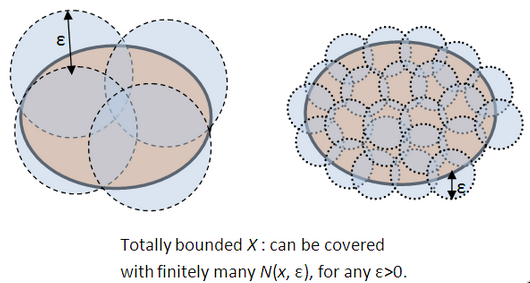
\includegraphics[width=0.8\textwidth]{assets/compact_set_ex.png}
  \caption{Compact Set}
  \label{fig:compact_set_ex}
\end{figure}

\begin{definition}
  A subset $E \subseteq X$ is \textbf{bounded} if  $\exists x_0 \in X, r >0$, such that  $E \subseteq B_r(x_0)$
\end{definition}

\begin{prop}
  If $E \subseteq X$ is \textbf{compact} then E is \textbf{bounded}
  \begin{proof}{By Contradiction}\\
    Assume that $E$ is compact but not bounded.  Take $x_0 \in X$ and consider the open cover of $E$,  $U_n = B_n(x_0)$ 
    for $n=1,\ldots,n$. We know that each of these balls $B_n(x_0)$ is open by definition. Then $E \subseteq \cup_{n \geq 1} B_n(x_0)$.
    Since $E$ is compact, then there exists finite subcover, so $\cup_{n \geq 1} B_n(x_0)$ is composed of finitely many balls.
    Then, $\exists 1 \leq n_1 < n_< \ldots < n_k$ such that $E \subseteq \cup_{j=1}^k B_{n_j}(x_0) = B_{n_k} (x_0)$ 
    and $E$ is contained in a ball with largest radius and this means $E$ is bounded which is a contradiction!  \end{proof}
\end{prop}
\begin{note} 
    In this proof, we are constructing a finite subcover of concentric balls starting from the origin with increasing radius,
    one possible out of many.
\end{note}

\begin{definition}
  The \textbf{haussdorff property} is defined as follows. For any $x \neq y$ in  $\left( X, \rho \right) $ metric space.
  Then $\exists r>0$ such that $B_{r_1}(x) \cap B_{r_2}(y) = \emptyset$. This \textbf{Haussdorff space} is also known
  as the \textbf{T2 axiom}.
\end{definition}
\begin{note}
  This is always true for \textbf{metric spaces}

  \begin{proof}{By contradiction} \\
    Take $0 < r < \frac{\rho(x,y)}{2}$. Assume $\exists z \in X$ such that $z \in B_r(x) \cap B_r(y)$.  Then,
    by the triangle inequality:
    \[
    \rho(x,y) \leq \rho(x,z) + \rho(z,y) < r + r = 2r 
    .\] 
    \[
    \frac{\rho(x,y)}{2} < r
    .\] 
    However, this contradicts the assumption $0 < r < \frac{\rho(x,y)}{2}$. Therefore, such a point $z$ 
    cannot exist. Any metric space must be haussdorff.
  \end{proof}
\end{note}

\begin{prop}
  If $E \subseteq X$ is compact then is a closed set in $X$. 

  \begin{proof}
    Assume that $E$ is compact. We will use the fact that we already proved if a set $U$ is open, then it's complement
    $U^c$ is closed. So we will show $X \setminus E$ is an open set. If $E = X$ then  $E$ is closed since it is 
    the whole metric space and metric spaces are closed sets. Assume $E \neq X$. Then, take  $x \in X \setminus E$.
    For any $y \in E$,  $\exists r_y > 0$ such that $B_{r_y}(x) \cap B_{r_y}(y) = \emptyset$. Then,
    $\{B_{r_y} (Y)\}_{y \in E} $ is an open cover of $E$ (in fact, even the centers would cover $E$). Since
    $E$ is compact  $\exists y_1, \ldots, y_N \in E$ such that $E \subseteq \cup_{j=1}^N B_{r_{y_j}}$, a finite
    subcover.  Take $r = min \{r_{y_i}, r_{y_2}, \ldots, r_{y_N}\} > 0$. This means $\forall 1 \leq j \leq N$:
     \[
    B_r(x) \cap B_{y_j}(y_j) \subseteq B_{r_j} (x) \cap B_{r_j}(y_j) = \emptyset
    .\]
    So,
    \[
      B_r(x) \cap (\cup_{j=1}^N B_{r_j}(y_j)) = \emptyset
    .\] Then,
  $B_r(x) \cap E = \emptyset$ and  $B_r(x) \in X \setminus E$. Since we can make this argument for any
  $x \in X \setminus E$, then $X \setminus E$ is open. And $E$ must be closed set in $X$.
  \end{proof}
\end{prop}

\begin{prop}
  Let $E \subseteq X$ compact and  $A \subseteq E$ and $A$ closed in  $X$. Then, $A$ is compact in $X$. 
  \begin{proof}
  Let $\{ U_\alpha\}_{\alpha \in I}$ be an open cover of $A$. We will prove that it has a finite subcover. 
    Since $A$ is closed, then  $X \setminus A$ is open and we get $\{\{U_{\alpha}_{\alpha \in I} , X \setminus A \} \}$
    which is an open cover of $E$. Since  $E$ is compact,  $\exists $ a finite subcover of $E$, 
    $\{U_{\alpha_1}, U_{\alpha_2}, \ldots, U_{\alpha_N}, X\setminus A\}$. Then, $\{U_{\alpha_1}, \ldots, U_{\alpha_N} \}
     \subseteq \{U_{\alpha_1}, U_{\alpha_2}, \ldots, U_{\alpha_N}, X\setminus A\}$ and is a finite subcover of
    $A$.  
  \end{proof}
\end{prop}

\begin{prop}
  Let $E$ be a compact set and let  $S \subseteq E$ compact that has infinitely many element. Then  $\exists $
  a limit point of $S$ inside $E$. (will be used later on when talking about convergence).
  \begin{proof}{By Contradiction}\\
    Assume $E$ is compact and  $S \subsete E$ and  $S$ has infinitely many points and  $S$ does not have a 
    limit point in  $E$. This means that since $S \subseteq E$, if there is no limit point in $E$,
    then $S$ does not have a limit point in general. Then for $\forall y \in E$ we have that  $y$ is not
    a limit point of  $S$ meaning, 
     \[
        \forall y \in E, \exists r_y > 0 \text{ such that } B_{r_y} (y) \text{ contains only finnitely many points from S}
    .\] 
    Then, 
    \[
    \{B_{r_y} \left( y \right) \}_{y \in E}
    .\] 
    is an open cover of $E$. Since $E$ is compact, $\exists $ a finite subcover of $E$:
     \[
       \{ B_{r_{y_1}} (y_1), \ldots, B_{r_{y_N}}(y_N) \} \text{ where } y_1,\ldots,y_N \in E 
     .\] 
     Then, $E \subseteq \cup_{i=1}^N B_{r_{y_j}}(y_j)$ and since $N$ is a finite number and for each  $B_{r_{y_j}}(y_j)$ 
     there only exist finitely many elements from $S$, then this means that $|E|$ is finite and since $S \subseteq E$,
      $S$ has only finitely many elements, but this is a contradiction!
  \end{proof}
\end{prop}

\section{Characterization of Compact Sets in $\R^n$}

\subsection{Suprenum and Infinitum in $\R$}
\begin{definition}
  M is an \textbf{upper bound} of $E \subseteq \R$ if $\forall x \in E$,  $x \leq M$
\end{definition}

\begin{definition}
  Let  $E \subseteq \R$ and let $E$ be bounded above (i.e.  $\exists $ an upper bound of $E$), then
  $alpha = sup(E)$ is known as the \textbf{suprenum} of $E$ if it satisfies:
    \begin{enumerate}
     \item $\alpha$ is an upper bound
     \item  $\forall \epsilon > 0$, the interval $(\alpha - \epsilon, \alpha] \cap E \neq \emptyset$
   \end{enumerate}
\end{definition}

\begin{remark}{Maximum vs Suprenum} \\
  Maximum can be thought of as the suprenum that belongs to the set. However, \textbf{the suprenum may not 
  necessarily belong to the set} (think limits). The same holds for the minimum and infinitum.
\end{remark}

\begin{definition}
  Then the infinitum $\beta = inf(E)$is defined as:
  \begin{enumerate}
    \item $\beta$ is a lower bound
    \item  $\forall \epsilon > 0$, the interval  $[\beta, \beta + \epsilon) \cap E \neq \emptyset$ 
  \end{enumerate}
\end{definition}

\begin{figure}[h]
  \centering
  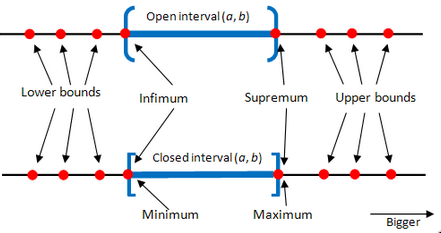
\includegraphics[width=0.8\textwidth]{assets/sup_inf_ex.png}
  \caption{Suprenum and Infinitum vs Maximum and Minimum}
  \label{fig:sup_inf_ex}
\end{figure}

\begin{theorem}
  If $E \subseteq \R$ is bounded above then $\exists $ $sup(E)$. A similar statement holds for  $inf(E)$ 
  if  $E$ is bounded below.
\end{theorem}

\begin{prop}
The $sup(E)$,  $E$ is bounded above, is unique.
\begin{proof}{By Contradiction} \\
  Assume that there exists two suprenum $\alpha_1, \alpha_2$, $\alpha_1 \neq \alpha_2$. Then WLOG, let
  $\alpha_1 < \alpha_2$. This means that for $\alpha_1$ in  $E$, by definition,  $\exists \epsilon_1$ 
  such that the interval $(\alpha_1 - \epsilon_1, \alpha_1] \cap E \neq \theta$ and for $\alpha_2$ in $E$,
  $\exists \epsilon_2$ such that $( \alpha_2 - \epsilon_2, \alpha_2 ] \neq \theta$. However, because 
  $\alpha_1 < \alpha_2$ then $\alpha_1 \in ( \alpha_2 - \epsilon_2, \alpha_2 ]$ which is non-empty with intersection
  with $E$, so there are elements  $\alpha_1 < \alpha_1 + \epsilon_1 \in E$. This means that $\alpha_1$ 
  is not an upper bound and can't be a suprenum! 
\end{proof}
\end{prop}

\begin{prop}
  If  $M$ is an upper bound of  $E \subseteq \R$ then $sup(E) \leq M$.
   \begin{proof}
    
  \end{proof}
\end{prop}

\begin{lemma}
  Let $I_1 \supseteq I_2 \supseteq \ldots \supset I_k \supseteq \ldots$ be a sequence of closed intervals
  \[
    I_k = [a_k,b_k] \subseteq \R \text{ for all } k=1,2, \ldots
  .\] 
  Then, 
  \[
  \cap_{k=1}^\infty I_k \neq \emptyset
  .\] 
  \begin{proof}
    Assume $I_1 \supseteq I_2 \supseteq \ldots \supset I_k \supseteq \ldots$ are closed intervals. 
    Then for any given $k \geq 1$,  $a_l \leq b_k$,  $\forall l \geq 1$ (i.e. all the "lower bound"'s are smaller 
    than any "upper bound"). Then $b_k$ is an upper bound of  $\{a_1,a_2, \ldots\}$ so through \textit{Theorem 1}:
     $\alpha = sup_{l \geq 1} \{a_l\}$ exists and  
     \[
       \alpha \leq b_k \forall k \in 1,2,\ldots  
     .\]. Then, $\alpha$ is a lower bound for  $\{b_k | k \in \N\}$. And by \textit{theorem 1} again,
     \[
     \exists \beta = inf \{b_k | k \in \N\}  
     .\] 
     and, $\alpha \leq \beta$. Then, $\forall k \in \N$,
     \[
       a_k \leq \alpha \leq \beta \leq b_k \iff [\alpha, \beta] \subseteq I_k 
     .\] 
     So, 
     \[
       \cap_{k=1}^{\infty} I_k \supset [\alpha, \beta]
     .\]
     and the intersection is non-empty as $[\alpha, \beta]$ contains at least 1 element (when  $\alpha = \beta$)
  \end{proof}
\end{lemma}

\begin{note}
  If the intervals were not closed. For example: $I_n = \left( 0, \frac{1}{n} \right) $ for $n=1,2,3,\ldots$,
  then $\cap_{n \geq 0} I_n = \emptyset$
\end{note}

\begin{theorem}
  If $a \leq b$, then  $I = [a,b] \subseteq \R$ is compact.

  \begin{proof}{By contradiction}\\
    Assume that $I$ is not compact, then  $\exists $ an open cover $\{ U_{\alpha}\}_{\alpha \in A}$ of the interval
    $I$ that does not have a finite subcover. Take the midpoint of the interval $\frac{a+b}{2}$ and split $I_1 = I$ into
    $$I_1' = [a,\frac{a+b}{2}]$$ and $$I_1'' = [\frac{a+b}{2}, b]$$. One of these intervals cannot be covered by
    finitely many sets from the collection $\{U_{\alpha}\}_{\alpha \in A}$, otherwise if both could be covered
    by finitely many, then $I$ would have a finite subcover. Let us call this non-finitely covered interval $I_2 \subseteq I_1$.
    Continuing with this process for $I_n$, we construct $I_1 \supseteq I_2 \ldots \supseteq I_k \supseteq \ldots$,
    where:
    \begin{enumerate}
      \item $I_k \supset I_{k+1} \forall k \geq 1$
      \item $\forall k \geq 1, I_k$ can not be covered by finitely many sets from  $\{U_{\alpha}\}_{\alpha \in A}$ 
      \item $\mid I_k\mid  = \frac{b-a}{2^{k-1}}, k = 1,2,\ldots$
    \end{enumerate}
    By \textit{Lemma 1}, $\exists x \in \cap_{k=1}^\infty I_k$. Then $\exists \beta \in A$ such that $x \in U_{\beta}$.
    Since $U_\beta$ is open,  $\exists \epsilon > 0$ such that  $U_{\beta} \supseteq \left( x - \epsilon, x + \epsilon \right)$ for
    some $\epsilon > 0$. It now follows from property (3), that $\exists k \geq 1$ such that $I_k \subseteq \left( x - \epsilon,
    x + \epsilon \right) \subseteq U_\beta$. This is a contradiction with property (2) because $I_k$ can be covered by  $\{U_\beta\}$ 
    which is a finite subcover of size 1! Thus, $I = [a,b]$ is compact
  \end{proof}
\end{theorem}

\section{Compact Sets in $\R^n$}
Consider the rectangular box $I_n$:
\[
  [a_1,b_1] \times [a_2, b_2] \times \ldots \times [a_n,b_n] = \{\left( x_1,\ldots,x_n \right) \in \R^n | 
  a_k \leq x_k \leq b_k \forall k = 1,2,\ldots\} 
.\] 

\begin{theorem}
  $n \geq 1, I^n$ is bounded in $\R^n$
  The proof follows the argument in theorem (2) 
\end{theorem}

\begin{theorem}
$E \supseteq \R^n$ is compact $\iff E$ is closed and bounded.
\begin{proof}
   $\rightarrow$: Since $E$ is compact  $\to$  $E$ is closed and bounded by prop 1 and 2. \\

   $\leftarrow$: Assume that $E$ is closed and bounded in  $\R^n$. Then $\exists $ a rectangular box $B$ 
    inside $\R^n$ such that $E \subseteq B$ (we can consider the ball centered at $E$, then draw a box around it).
    But now realize that $E$ is closed and  $B$ is compact (by theorem 3) and by Proposition 3, this means that
    $E$ is compact. \\
\end{proof}
\end{theorem}

\begin{note}
  The above is not true in general, i.e. $E \subseteq X \not\iff$ E is closed and bounded. For example, consider
  $X = [0,1)$ and  $\rho(x,y) = \mid x-y\mid $, so $(X, \rho)$ is the metric space. Define  $E= [\frac{1}{2},1)$.
  Then $E$ is closed and bounded  in $ X$. But $E$ is not compact. Consider the open cover of E,
   \[
   U_k = \left( 0, 1 - \frac{1}{k+2} \right)  k = 1,2,3,\ldots 
   .\]
   Then, $\cup_{k \geq 1} U_k \supseteq E$. But this open cover does not have a finite subcover that covers $E$!
   \[
   \lim_{k \to \infty} U_k = \left( 0, 1 \right) 
   .\] 
   So there is no way to contain $\left( 1 - \epsilon,1 \right) \subseteq E$ as $\epsilon \to 0$ with finite subsets, it gets
   closer and closer but never reaches. 
\end{note}


\end{document}
